\section{Nested sampling setup}

Here we will briefly describe some of the core functions used for the Nested Sampling algorithm within our code. We will
not describe nested sampling itself, over-and-above the very brief summary given in \S\ref{sec:general}, but instead refer
the reader to \citet{Veitch:2010}. We also refer the reader to \citet{2015PhRvD..91d2003V} for a more thorough description
of some of the concepts we will discuss below.

One main point about the nested sampling algorithm is that it starts by randomly drawing a certain number of samples (the number of
which we call the number of live points, $N_{\text{live}}$, which will be the constant number of ``active'', or ``live'', samples),  
where a sample is a vector containing a value for each parameter $\vec{\theta}$, from the prior distribution (see \S\ref{sec:priorfuncs}).
The samples must be independent draws. For each of these samples the likelihood will be calculated and the sample $\vec{\theta}_{\text{min}}$
corresponding to the minimum likelihood, $L_{\text{min}} = p(\mathbf{B}|\vec{\theta}_{\text{min}})$, will be noted. As the algorithm
progresses the number of live points stays the
same, but at each iteration a new sample will be added in place of the one with the minimum likelihood, and therefore the
minimum likelihood will continuously be updated to be the minimum value for the current set of points.

\subsection{Proposal functions}\label{sec:proposals}

The nested sampling algorithm requires a way to draw new samples from the parameter space that is being explored. The
particular requirement for nested sampling is that any new sample is an independent draw from a constrained version
of prior probabilty function for each parameter. The constraint is that the new sample's likelihood must be greater
than the current value of $L_{\text{min}}$, e.g. for a single parameter $x$, the probability of drawing a point at $x_i$ 
would be
\begin{equation}
 p(x=x_i|I)_{\text{constrained}} = \begin{cases}
             p(x=x_i|I) & \text{if~} p(\mathbf{B}|x_i) > L_{\text{min}}, \\
             0 & \text{otherwise},
            \end{cases}
\end{equation}
where $p(x|I)$ is the prior on $x$.

There are various methods to sample from the constrained prior, the simplest of which is just to sample from the full
prior and only accept a sample if it meets the likelihood constraint. However, such a simple method soon becomes very
inefficient if the likelihood gets more and more tightly concentrated within the prior volume (which can happen rapidly
for high-dimensional problems). One popular nested sampling method is MultiNest \citep{2009MNRAS.398.1601F}, which performs
the sampling by calculating a set of ellipsoids bounding the live points and drawing points uniformly from within them.
Various other approaches exist such as Diffusive Nested Sampling \citep{Brewer2011,2016arXiv160603757B} and POLYCHORD \citep{2015MNRAS.450L..61H}.

The version of nested sampling used in the \lalinf library, as used by our code, makes use of a Markov chain Monte Carlo (MCMC) approach to
drawing new samples \citep{Veitch:2010}. The MCMC attempts to sample from the constrained prior distributions in an efficient manner, with
the final sample of the chain being a statistically independent sample from the rest of the live points. To sample most efficiently
the MCMC requires a proposal distribution that closely resembles the underlying constrained prior that it is trying to sample from.
\lalinf has a variety of potential proposal distributions \citep{2015PhRvD..91d2003V}, but our code currently allows five different
proposals, that can be used in different proportions:
\begin{description}
 \item[Ensemble walk] This is one of the affine invariant ensemble proposals described by \citet{GoodmanWeare}, which adopt the
 scale and shape of the current set of samples. The hard-coded setup in \lalinf is that three samples randomly drawn from a cache
 of samples are used to define the ``walker'' samples. This is the main default proposal of our code, and is used as the proposal
 75\% of the time.
 \item[Ensemble stretch] This is another affine invariant ensemble proposal described by \citet{GoodmanWeare}, and makes use of
 two samples randomly drawn from the sample cache. By default this proposal is not used at all.
 \item[Differential evolution] This is similar to the stretch proposal in that it uses two samples randomly drawn from the sample
 cache. By default this proposal is not used at all.
 \item[Uniform proposal] This proposal just draws points from their full prior for parameters that have a uniform prior specified.
 This proposal is used 25\% of the time by default.
 \item[Frequency jump] This proposal tries jumping between Fourier frequency bins if frequency is one of the required parameters.
 This proposal has not been tested and, by default, is not used at all.
\end{description}
The cache of samples mentioned above, and used by the nested sampling algorithm, is the set of live points, but this cache is
only updated on iterations of the algorithm that are a factor of 10\% of the number of live points.

The length of each MCMC run can be chosen by the user, but by default it is automatically set within the code. To do this,
at the same rate as the cache is updated, the autocorrelation length of the parameters is calculated. A random sample from the current
live points in chosen, and evolved via the MCMC, and the autocorrelation length of each parameter is calculated, $\vec{{\text{acl}}}$. The number
of MCMC iterations, $n_{\text{MCMC}}$, is then chosen as $n_{\text{MCMC}} = \text{min}(\text{max}(\vec{\text{acl}}), 5000)$, where 5000 is
a hardcoded maximum length.

\subsubsection{Testing the proposals}\label{sec:proposaltesting}

We would like to test whether some of the above proposals lead to accurate calculations of the evidence integral as given in Equation~\ref{eq:evidence}.
It is especially interesting to do this over ranges of prior volumes that are initially similar to the posterior volume, but then diverge to be
much larger than the posterior volume (or in other words, as the information gain, $H$, or Kullback-Leibler divergence, increases). To do this our
code has the option of setting a one-dimensional Gaussian distribution as the likelihood function, using a flat prior bounded between $A$ and $B$,
and working out the evidence. Analytically the evidence is given by
\begin{align}\label{eq:testgaussev}
 \mathcal{Z} &= \int_A^B \frac{1}{\sqrt{2\pi}\sigma}\exp{\left(-\frac{(x-\mu)}{2\sigma^2} \right)}\frac{1}{(B-A)} \text{d}x, \nonumber \\
   &= \frac{1}{2(B-A)}\left(\erf{\left[\frac{(\mu-A)}{\sqrt{2}\sigma}\right]}-\erf{\left[\frac{(\mu-B)}{\sqrt{2}\sigma}\right]}\right).
\end{align}
As we are often interested in setting upper limits of, for example, the \gw amplitude $h_0$, we can also use the test to see if the
upper limits we obtain from the posterior samples match the expected upper limit obtained (via root finding) from the CDF of the distribution
\begin{equation}\label{eq:testcdf}
 \text{UL}(x) = \frac{1}{2a}\left(\erf{\left[\frac{(\mu-A)}{\sqrt{2}\sigma}\right]} - \erf{\left[\frac{(\mu-x)}{\sqrt{2}\sigma}\right]}\right),
\end{equation}
where $a = (\erf{\left[(\mu - A)/\sqrt{2}\sigma\right]} - \erf{\left[(\mu - B)/\sqrt{2}\sigma\right]})/2$ is the area under the distribution.
We can calculate the true Kullback-Leibler divergence via
\begin{widetext}
\begin{align}\label{eq:kldiv}
H =& \int_A^B p(x|\mu,\sigma,I) \ln{\left(\frac{p(x|\mu,\sigma,I)}{p(x|I)}\right)} \text{d}x, \nonumber \\ 
 =& \int_A^B \frac{p(\mu,\sigma|x,I)p(x|I)}{\mathcal{Z}} \ln{\left(\frac{p(\mu,\sigma|x,I)p(x|I)}{\mathcal{Z}p(x|I)}\right)} \text{d}x, \nonumber \\
 =& \frac{p(x|I)}{\mathcal{Z}} \int_A^B p(\mu,\sigma|x,I) \left[\ln{\left( p(\mu,\sigma|x,I) \right)} - \ln{\mathcal{Z}}\right] \text{d}x, \nonumber \\
 =& -\frac{p(x|I)}{4\mathcal{Z}}\Bigg[ \left(1+2\left(\ln{\mathcal{Z}} 
+\ln{\left[\sqrt{2\pi}\sigma\right]}\right)\right)\left(\erf{\left(\frac{\mu-A}{\sqrt{2}\sigma}\right)}-\erf{\left(\frac{\mu-B}{\sqrt{2}\sigma}\right)} \right) + \nonumber \\
 & \frac{2}{\sqrt{2\pi}\sigma}\left((A-\mu)\exp{\left(-\frac{(A-\mu)^2}{2\sigma^2}\right)} - (B-\mu)\exp{\left(-\frac{(B-\mu)^2}{2\sigma^2}\right)}  \right) \Bigg]
\end{align}
\end{widetext}
where $p(x|\mu,\sigma,I)$ is the posterior, $p(\mu,\sigma|x,I)$ the likelihood, and $p(x|I)$ is the prior (with $p(x|I) = (B-A)^{-1}$), and $\mathcal{Z}$ is the
evidence calculated via Equation~\ref{eq:testgaussev}. For the case of $\mu=0$ and $A=0$, and provided $B \gg \sigma$, this generally simplifies
to
\begin{equation}
H \approx -\frac{1}{4\mathcal{Z}B}\left[1+2\left(\ln{\mathcal{Z}} +\ln{\left(\sqrt{2\pi\sigma^2}\right)}\right)\right].
\end{equation}
A final thing that we can check, on top of the upper limit value, is whether the posterior samples appear to be drawn from the expected
posterior distribution. To do this we use a Kolmogorov-Smirnov test comparing the CDF of the samples with the analytical CDF and calculating the
two-sided $p$-value for the null hypothesis that the two distributions are the same.

In the tests below we have run the code on this Gaussian likelihood with a Gaussian of zero mean and $\sigma = 10^{-24}$, truncated at zero
by fixing the lower prior bound to $A=0$. This is similar to the form of the likelihood seen in pulsar searches when no signal is present.
We have then set a range of upper bounds, $B$, from $10^{-23}$ to $10^{-13}$ increasing by a factor of ten each time, and a range of numbers of
live points from $2^9$ to $2^{13}$ increasing by powers of two each time. For each combination of upper bound and number of live points we have
run the code on the test Gaussian likelihood 100 times to see the statistical spread of the output.

In the first test we check how just using the ensemble walk proposal (which is {\it not} the default configuration described above) fairs at
estimating the evidence, upper limit, and posterior distribution. Figure~\ref{fig:walkpropevs} shows a variety of information, but it
primarily shows the distribution of the ratio of evidences output from our code, $\mathcal{Z}$, to the true evidence calculated via
Equation~\ref{eq:testgaussev} as a function of the value of the upper prior bound $B$ (or equivalently on the top axis the
information gain, in nats, calculated via Equation~\ref{eq:kldiv}). This is shown for the range of different numbers of live points used.
It is clear that as the information gain increases (i.e.\ the posterior is constrained within a successively smaller part of the
prior range) we are systematically more biased towards overestimating the evidence. It can also be seen that the bias increases with
increasing number of live points. Linear fits (in $\ln{(\mathcal{Z}/\mathcal{Z}_{\text{true}})}$ and $H$, the information gain) for different numbers
of live points are shown in Table~\ref{tab:klvsz}. It is interesting to note that the statistical spread of values (if ignoring the
systematic offset) are consistent with the expected range given by the error bars, and calculated using $\sqrt{H/N_{\text{live}}}$, where here
$H$ is the mean of the {\it information gain} (in nats) returned by the nested sampling algorithm for each run.

\begin{table}[h]
\caption{Linear coefficients in fits of $\ln{(\mathcal{Z}/\mathcal{Z}_{\text{true}})} = mH + c$ from the results
shown in Figure~\ref{fig:walkpropevs} for differing numbers of live points.\label{tab:klvsz}}
\begin{center}
\begin{tabular}{l c c}
\hline
\hline
$N_{\text{live}}$ & $c$ & $m$ \\
\hline
512 & $-0.27$ & 0.045 \\
1024 & $-0.24$ & 0.058 \\
2048 & $-0.18$ & 0.065 \\
4096 & $-0.12$ & 0.068 \\
8192 & $-0.09$ & 0.070 \\
\hline
\end{tabular}
\end{center}
\end{table}

\begin{figure}[phtb]
\begin{center}
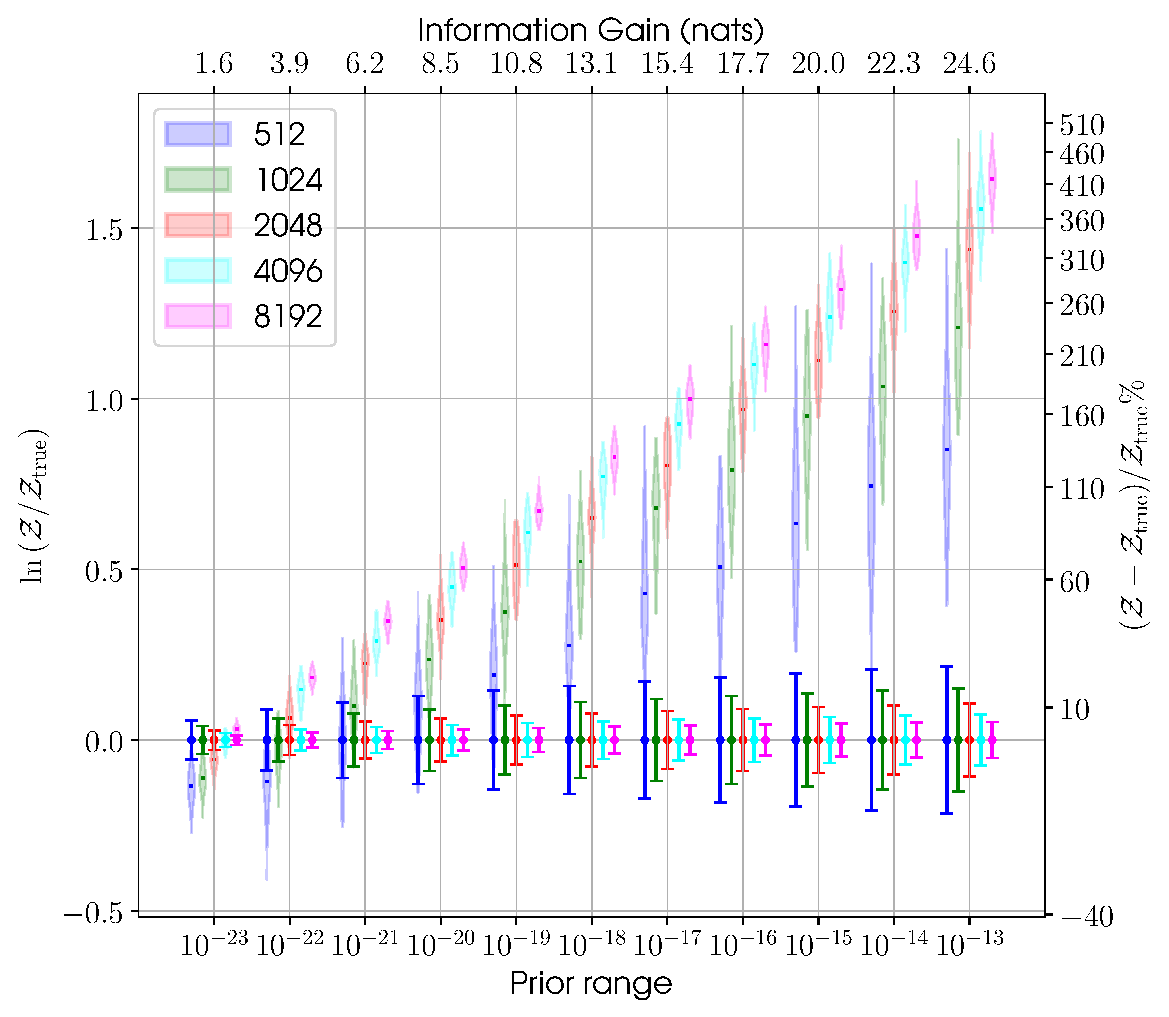
\includegraphics[width=1\columnwidth]{./figures/proptesting/walk_prop/evidences/collate_plots_wp_evidences}
\caption{ \protect\label{fig:walkpropevs}
A set of violin plots showing the distributions of estimates of the evidence
$\mathcal{Z}$ (as returned by our code) compared to the true evidence $\mathcal{Z}_{\rm true}$ (as
calculated using Equation~\ref{eq:kldiv}) as a function of the prior range,
or information gain, when using only the ensemble walk proposal
distribution. The different colour plots represent different numbers
of live points used. Offsets around the different prior range values are just used to avoid overlaps of the
distributions.
}
\end{center}
\end{figure}

\begin{figure}[phtb]
\begin{center}
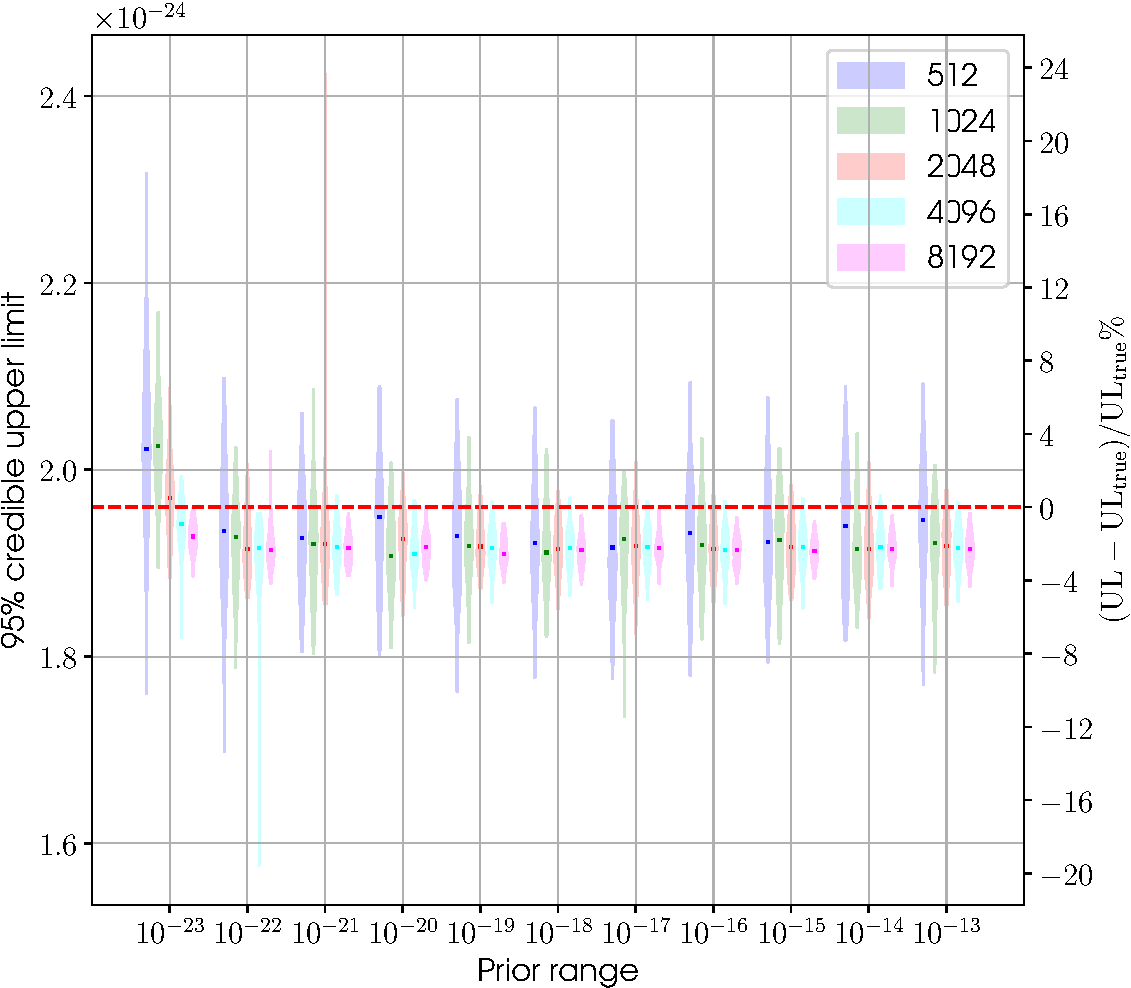
\includegraphics[width=1\columnwidth]{./figures/proptesting/walk_prop/upperlimits/collate_plots_wp_uls}
\caption{ \protect\label{fig:walkpropuls}
A set of violin plots showing the distributions of estimates of the 95\% upper limits on the Gaussian position parameter as a function of the prior range, when using only the ensemble walk proposal distribution. The different colours represent the different numbers of live points  used. The red dashed horizontal line shows the true analytical upper limit for the distribution.
Offsets around the different prior range values are just used to avoid overlaps of the
distributions.
}
\end{center}
\end{figure}

\begin{figure}[phtb]
\begin{center}
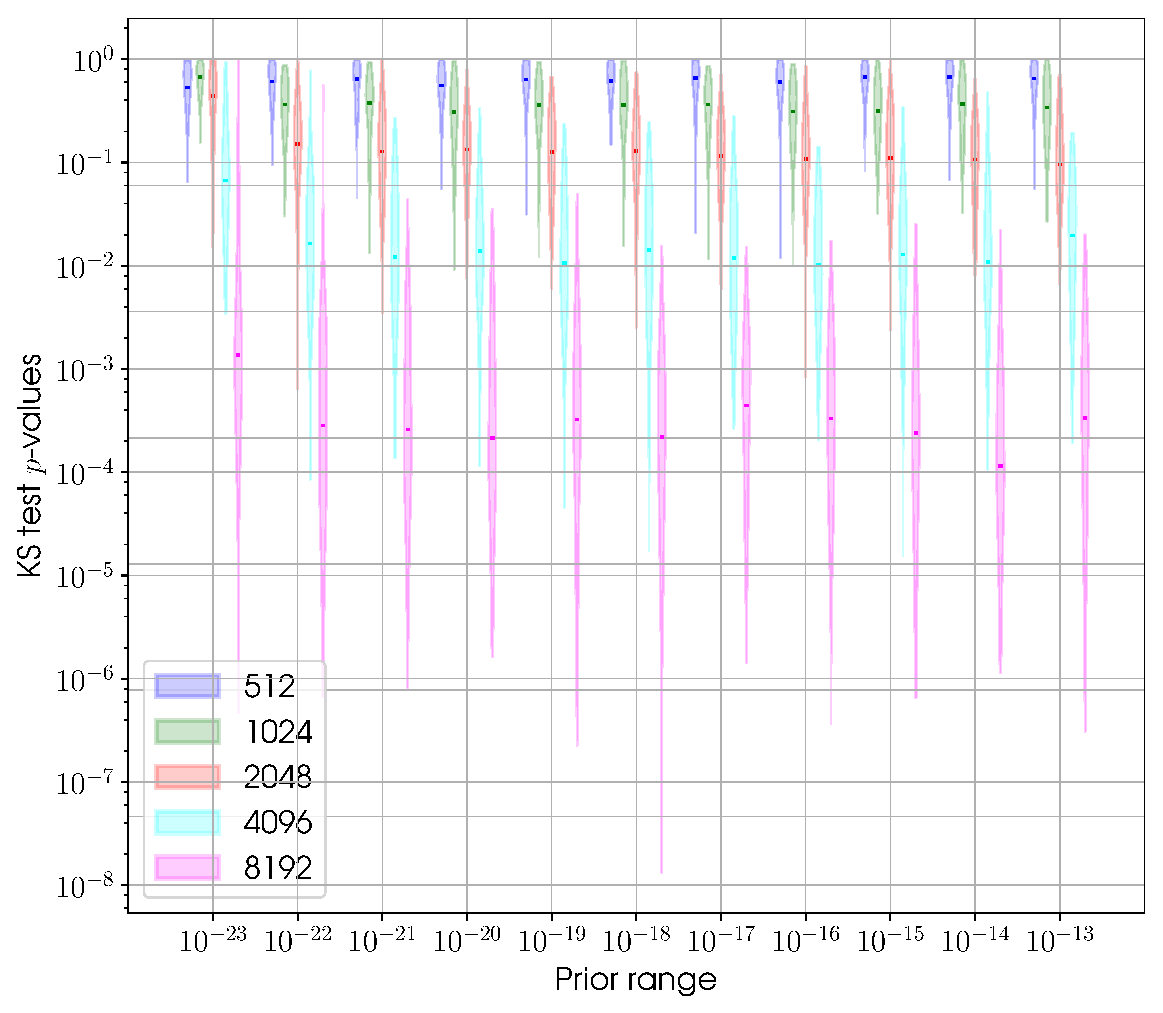
\includegraphics[width=1\columnwidth]{./figures/proptesting/walk_prop/kstest/collate_plots_wp_ks}
\caption{ \protect\label{fig:walkpropks}
A set of violin plots showing the distributions of Kolmogorov-Smirnov test
two-sided $p$-values comparing the posterior sample CDFs with the analytical
CDFs as a function of the prior range, when using only the ensemble walk proposal distribution. The different colour plot represent different numbers of live points used.
Offsets around the different prior range values are just used to avoid overlaps of the
distributions.
}
\end{center}
\end{figure}

Figure~\ref{fig:walkpropuls} shows the distribution of 95\% upper limits on the $x$ parameter in Equation~\ref{eq:testcdf} (calculated by solving
the equation for $\text{UL}(x) = 0.95$). It can be seen that, other than for the narrowest prior range, there is a systematic bias towards the
upper limit being underestimated by $\sim 2\%$. Figure~\ref{fig:walkpropks} show the distribution of two-sided $p$-values from a Kolmogorov-Smirnov
test comparing the CDF of posterior samples against the analytical CDF in Equation~\ref{eq:testcdf}. The $p$-value null hypothesis is that both
distributions are the same, and it should be noted that we performed 100 trials for each prior range value and number of live points. For the
lower numbers of live points the distributions appear to be consistent, however, for larger numbers of live points the distributions are rather
inconsistent a large amount of the time. This is most likely due to differences in distributions showing up more obviously when there are more
posterior samples to use.

The systematic biases in evidence values and upper limits may not be major problem, but does point towards there being some issue with the
implementation of the ensemble walk proposal.

In the second test we have check what happens with the code's current default proposal settings: using the ensemble walk proposal 75\%
of the time and the uniform proposal 25\% of the time. It should be noted that this default is not an accident, and came about from tests
similar to these when just using the ensemble walk proposal.

Figure~\ref{fig:walkunipropevs} shows the evidence distributions equivalent to those in Figure~\ref{fig:walkpropevs}. However, what can
be seen in this case is that there is no obvious systematic bias as a function of $H$, and the statistical uncertainty is
consistent with expectations (as shown by the error bars). Similarly, the upper limits and Kolmogorov-Smirnov $p$-values shown in
Figures~\ref{fig:walkunipropuls} and \ref{fig:walkunipropks} respectively are consistent. The reason why this combination of proposals
seems to work whereas the ensemble walk proposal on its own does not is currently not understood, but we plan more work on figuring this
out.

\begin{figure}[!phtb]
\begin{center}
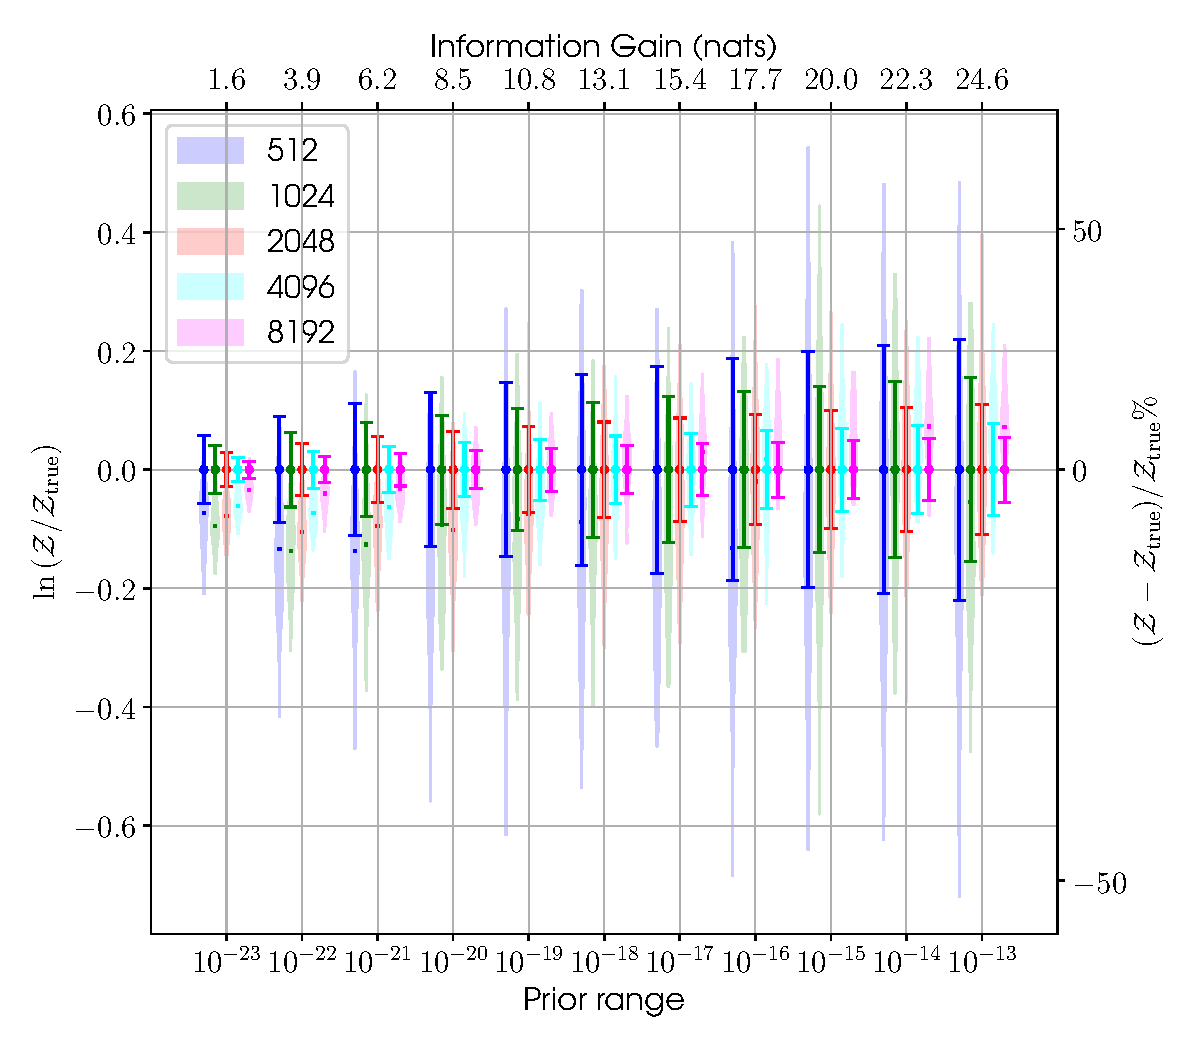
\includegraphics[width=1\columnwidth]{./figures/proptesting/walk_uniform_prop/evidences/collate_plots_wup_evidences}
\caption{ \protect\label{fig:walkunipropevs}
A set of violin plots showing the distributions of estimates of the evidence
$\mathcal{Z}$ (as returned by our code) compared to the true evidence $\mathcal{Z}_{\rm true}$ (as
calculated using Equation~\ref{eq:testgaussev}) as a function of the prior range,
or information gain, when using the ensemble walk and uniform proposal
distributions (75\% and 25\% of the time, respectively). The different colour plots represent different numbers
of live points used. The error bars show the expected spread of the log evidence ratios (calculated using
$\sqrt{H/N_{\text{live}}}$, where $H$ is the information gain from Equation~\ref{eq:kldiv}) if the average estimated
evidence match the true evidence. Offsets around the different prior range values are just used to avoid overlaps of the
distributions.
}
\end{center}
\end{figure}

\begin{figure}[!phtb]
\begin{center}
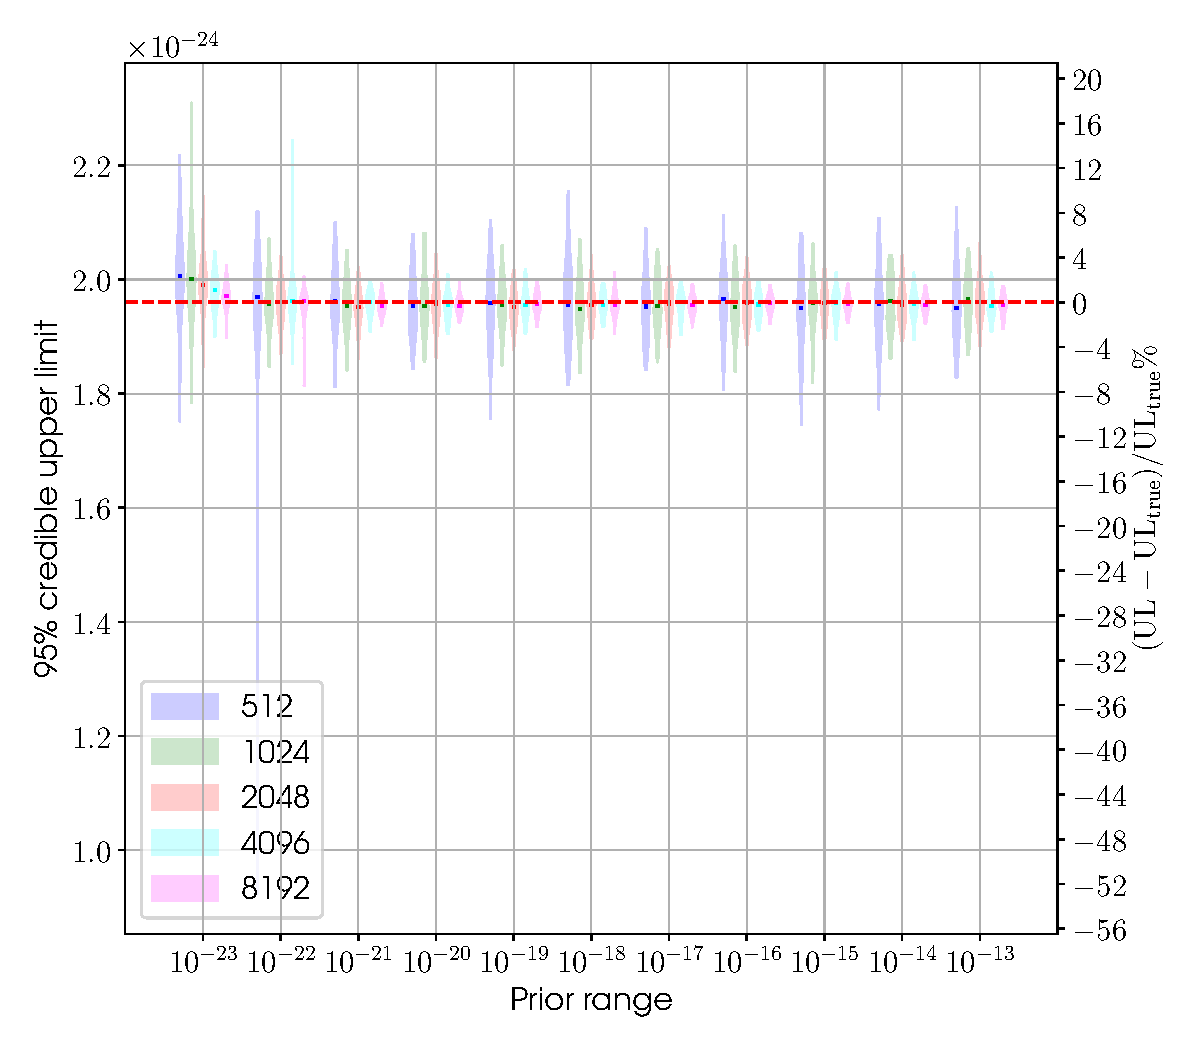
\includegraphics[width=1\columnwidth]{./figures/proptesting/walk_uniform_prop/upperlimits/collate_plots_wup_uls}
\caption{ \protect\label{fig:walkunipropuls}
A set of violin plots showing the distributions of estimates of the 95\% upper limits on the Gaussian position parameter as a function of the prior range, when using the ensemble walk and uniform proposal distributions. The different colours represent the different numbers of live points  used. The red dashed horizontal line shows the true analytical upper limit for the distribution.
Offsets around the different prior range values are just used to avoid overlaps of the
distributions.
}
\end{center}
\end{figure}

\begin{figure}[!phtb]
\begin{center}
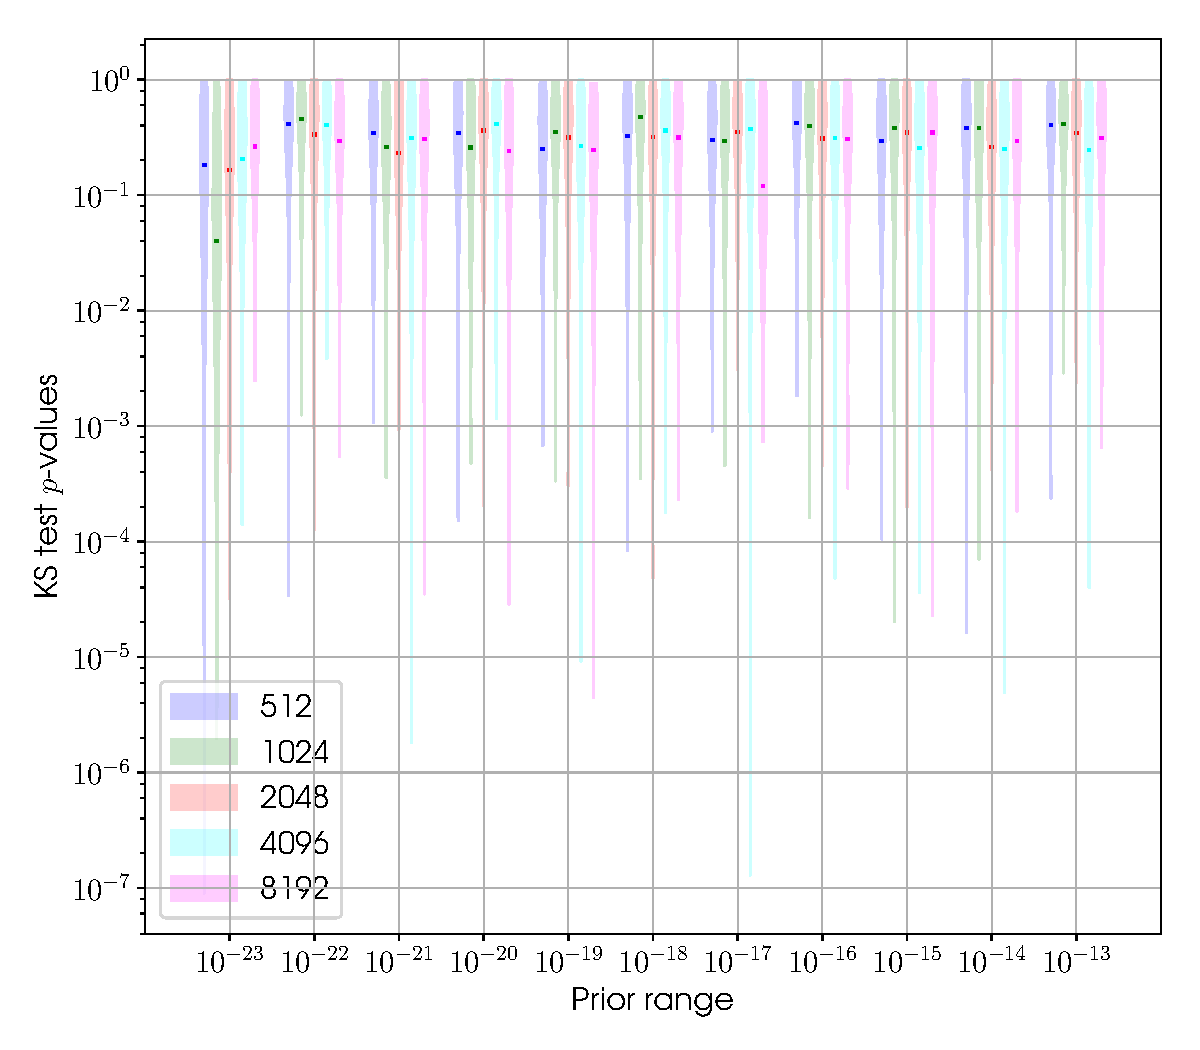
\includegraphics[width=1\columnwidth]{./figures/proptesting/walk_uniform_prop/kstest/collate_plots_wup_ks}
\caption{ \protect\label{fig:walkunipropks}
A set of violin plots showing the distributions of Kolmogorov-Smirnov test
two-sided $p$-values comparing the posterior sample CDFs with the analytical
CDFs as a function of the prior range, when using the ensemble walk and uniform proposal distributions. The different colour plot represent different numbers of live points used.
Offsets around the different prior range values are just used to avoid overlaps of the
distributions.
}
\end{center}
\end{figure}

\subsection{Posterior sample generation}\label{sec:postsamps}

As discussed in \S\ref{sec:general} nested sampling codes, such as \lppen, do not intrinsically output samples that can be histogrammed to give
representations of marginalised posterior distributions for the model parameters. They instead output an ascending likelihood ordered list of samples,
each of which occupies a known approximate amount prior volume. Samples must be drawn from these, with appropriate weighting (see Equation~\ref{eq:postaccept}),
to give a new set of samples that does represent the posterior distribution. During this process it is also possible to appropriately combine samples from parallel
independent nested sampling runs (weighting each based on their calculated evidences) to recalculate the evidence and generate posterior samples.

What is described above is not a core function of the \lppen code, but is an integral part to generating results with it, and has been used to
produce posterior distributions discussing earlier in the section, and later in this document. Due to the probabilistic
way that posterior samples are generated there will only be a finite number of samples, and the number of samples is dependent on the number
of live points used when running nested sampling. The actual dependence of the number of posterior samples on $N_{\text{live}}$ can be seen in
Figure~\ref{fig:numposts} (this uses the simulations discussed in \S\ref{sec:reseval}). It can be seen empirically, that the mean number of posterior
samples goes roughly as $\langle N_{\text{post}} \rangle \approx 2.4N_{\text{live}}$, although there is a lower tail extending to $N_{\text{post}} \approx
0.01N_{\text{live}}^{1.14}$.

\begin{figure}[!phtb]
\begin{center}
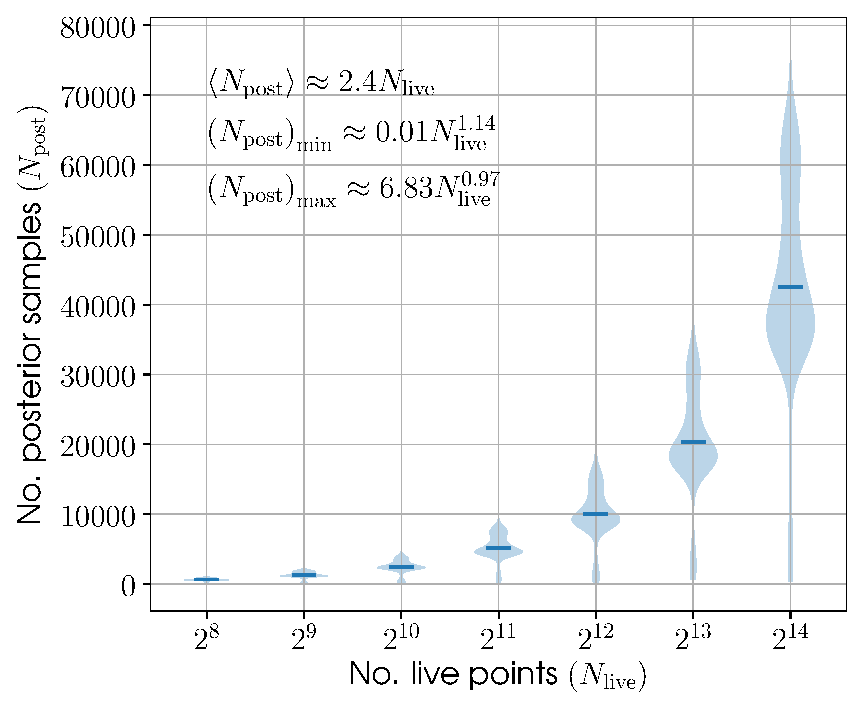
\includegraphics[width=1\columnwidth]{./figures/codeeval/stats/numposts/numposts}
\caption{ \protect\label{fig:numposts}
The distributions of the number of posterior samples produced as a function of the number of live points used in the nested sampling algorithm.
}
\end{center}
\end{figure}

\subsection{Code timing}\label{sec:timing}

How long the code takes to runs depends on two main factors: the number of live points used and the information gain going from prior to posterior. Increases
in both of these will generally mean that the code takes longer to run. Using the simulations from \S\ref{sec:proposaltesting} we have assessed the code
run time for the simple testing Gaussian likelihood function. This allows us to quantify the code run time as a function of both number of live points and information
gain.

We find that the median calculation time for the simple Gaussian likelihood function used in \S\ref{sec:proposaltesting} (on an Intel ``Haswell'' processor,
specifically Intel CPU E5-2680 v3 @ 2.50GHz), including some standard overheads\footnote{Without the overheads it is roughly $\sim 3.7\ee{-7}$ seconds.} is 
$\sim 5.9\ee{-6}$ seconds. The median time for calculation of the likelihood (including model calculation time) for a standard search (Eqn.~\ref{eq:stlikelihood})
over only non-phase evolution parameters, and for one chunk of data, is $8.1\ee{-5}$ seconds.\footnote{Without the additional overheads this is a similar time of
$4.9\ee{-5}$ seconds.}

The median run time per likelihood evaluation for the nested sampling part of the code for the standard likelihood function (using 1024 live points) 
is $8.5\ee{-4}$ seconds, which is $\sim 10$ times greater than the single likelihood evaluation time (this ratio will change as a function of the number
of live points). The median run time per likelihood evaluation for the nested sampling part of the code for the test Gaussian likelihood function
(using 1024 live points) is $1.8\ee{-4}$ seconds, which is $\sim 30$ times greater than the single likelihood evaluation time.

In Figure~\ref{fig:timings} we show the time taken for the runs in \S\ref{sec:proposaltesting},
using the default proposals, as a function of number of live points and information gain. The code run time is divided by $\mathcal{T}_{L}= 5.9\ee{-6}$ to
provide a way to scale it for other values of $\mathcal{T}_{L}$, e.g.\ that found from the code's standard likelihood function. If we perform a 2D linear
fit to the natural logarithm of the median run time, $R/\mathcal{T}_L$, we get the relation
\begin{align}\label{eq:runtime}
 \ln{\left(\frac{R}{\mathcal{T}_L}\right)} &\approx 1.57 \ln{N_{\text{live}}} + 1.05 \ln{H} + 3.60, \\
 \frac{R}{\mathcal{T}_L} &\approx 36.4 N_{\text{live}}^{1.57} H^{1.05}.
\end{align}
This relation should be considered as a rough lower limit to the run time for any particular likelihood function. Above, we saw that for our standard likelihood
function the nested sampling algorithm was roughly three times quicker per likelihood evaluation than the simple test function. In both cases the internal MCMC, which
draws new samples within the algorithm, required very similar small lengths to give uncorrelated samples, so there most be other internal bottlenecks that make the
simpler likelihood relatively slower. However, in general, longer MCMC chains will be required to give uncorrelated samples, so the number of likelihood evaluations
will increase.

\begin{figure}[!phtb]
\begin{center}
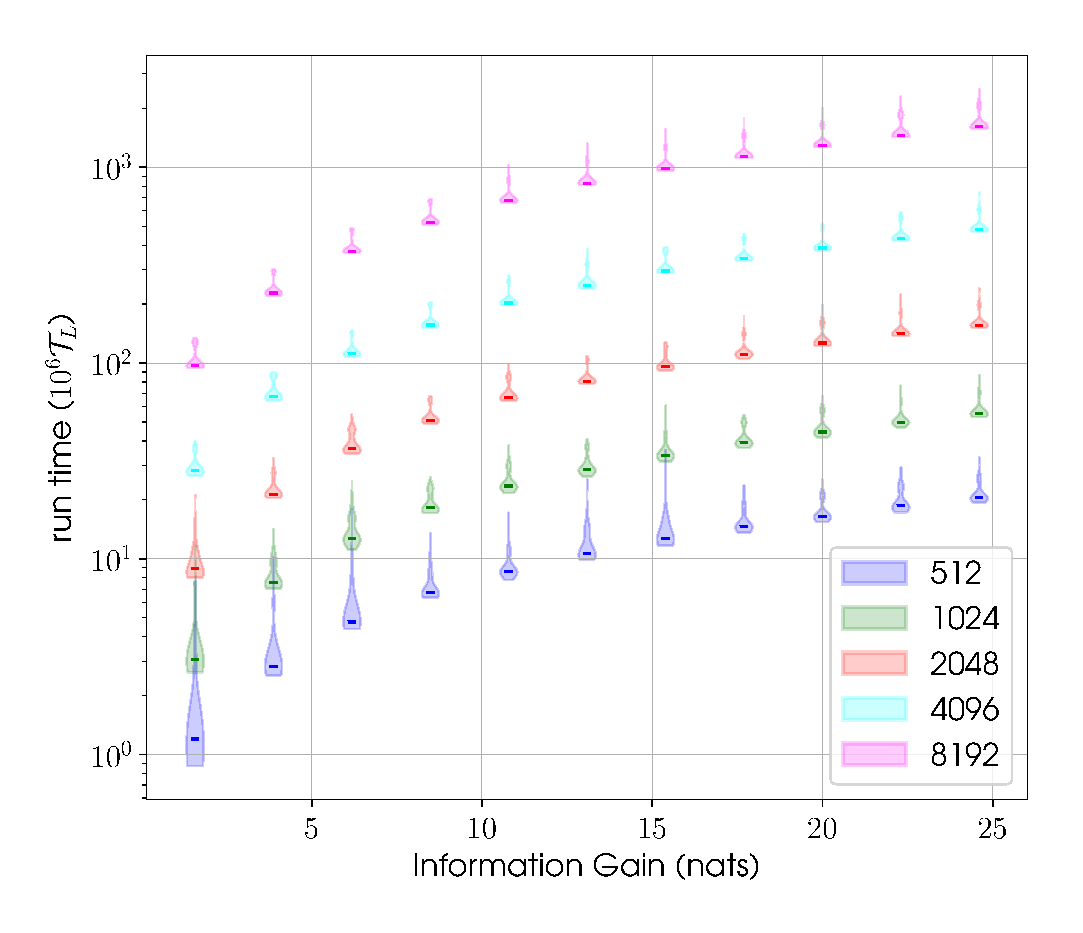
\includegraphics[width=1\columnwidth]{./figures/proptesting/walk_uniform_prop/timing/collate_plots_wup_timings}
\caption{ \protect\label{fig:walkpropks}
A set of violin plots showing the distributions of Kolmogorov-Smirnov test
two-sided $p$-values comparing the posterior sample CDFs with the analytical
CDFs as a function of the prior range, when using only the ensemble walk proposal distribution. The different colour plot represent different numbers of live points used.
Offsets around the different prior range values are just used to avoid overlaps of the
distributions.
}
\end{center}
\end{figure}
